\subsection{Time Aware traffic priorisation}

\begin{frame}{Transmission latency}
	\begin{columns}
		\column{0.3\textwidth}
		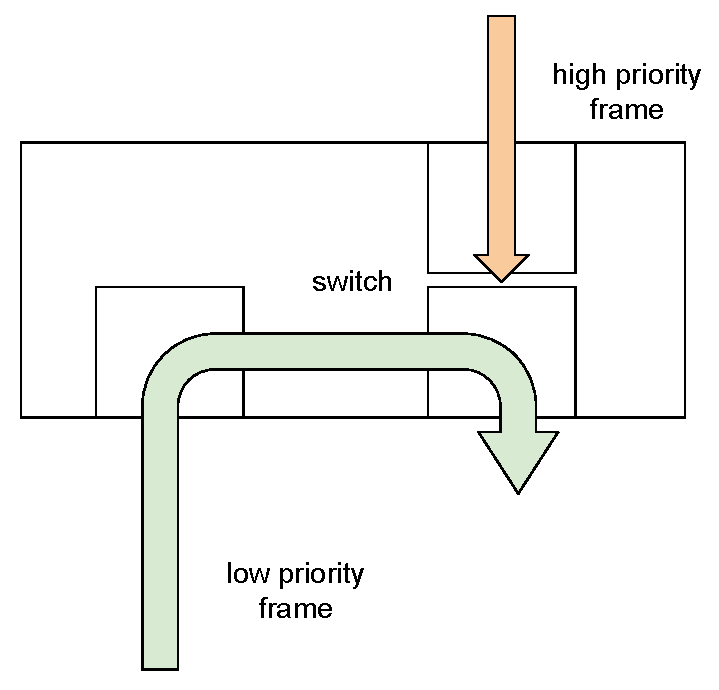
\includegraphics[width=1.1\textwidth]{slides/networking-tsn-taprio/switching_latency.pdf}
		\column{0.7\textwidth}
	\begin{itemize}
		\item Ethernet networks weren't originally designed for determinism
		\item Latencies can be introduced by on-device queues and buffers
		\item Bridges and switches can also introduce latencies
			\begin{itemize}
				\item In-flight frames can't be interrupted
				\item Low-priority frames need to be fully sent before high-priority frames launch
				\item At 100Mbps, 123 micro-seconds per frame
				\item At 1Gbps, 12,3 micro-seconds per frame
				\item Can happen for each switch on the Layer 2 network
			\end{itemize}
	\end{itemize}
	\end{columns}
\end{frame}

\begin{frame}{TC taprio}
	\begin{itemize}
		\item Allows creating \textbf{timeslots} and allocate them to \textbf{traffic classes}
		\item All devices on the network must agree on the timeslots
		\item \textbf{Guard periods} can be added to flush in-flight traffic
	\end{itemize}
	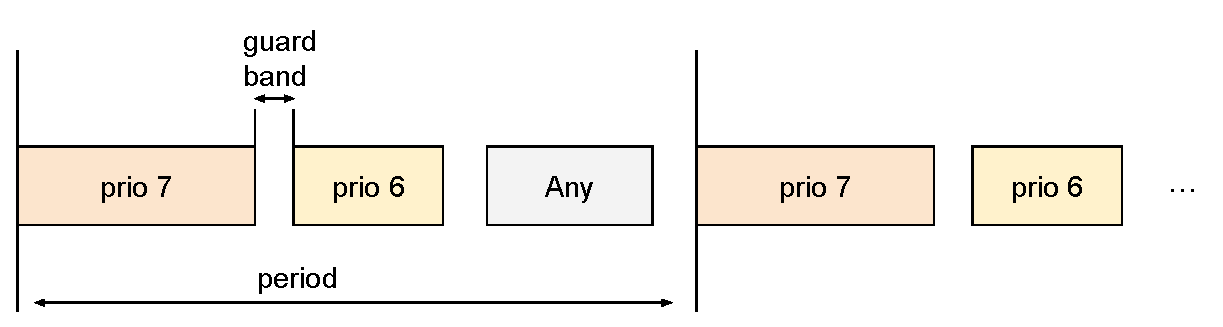
\includegraphics[width=\textwidth]{slides/networking-tsn-taprio/taprio.pdf}
\end{frame}

\begin{frame}[fragile]{TC taprio}
	\begin{block}{taprio example}
		\begin{minted}{bash}
tc qdisc add dev eth1 parent root handle 1 \
taprio num_tc 4 map 0 1 2 3 \
queues 1@0 1@1 1@2 1@3 base-time 1528743495910289987 \ # Start time
sched-entry S 0xff 200000000 \ # 200 ms for any class
sched-entry S 0x00 1000000 \ # 1 ms guard - class 0
sched-entry S 0x01 10000000 \ # 10 ms for class 1
sched-entry S 0x00 1000000 \ # 1 ms guard - class 0
sched-entry S 0x02 1000000 \ # 1 ms for class 2
sched-entry S 0x00 1000000 \ # 1 ms guard - class 0
sched-entry S 0x04 1000000 \ # 1 ms for class 3
sched-entry S 0x00 1000000 \ # 1 ms guard - class °0
clockid CLOCK_TAI
		\end{minted}
	\end{block}
\end{frame}

\begin{frame}[fragile]{TC ETF}
	\begin{itemize}
		\item Users specify a \textbf{launch time} for each packet
			\begin{itemize}
				\item The time is given using a reference clock
				\item Use \code{SO_TXTIME} and \code{sendmsg} with \code{SCM_TXTIME}
				\item A \code{delta} can be added to account for scheduling latency
			\end{itemize}
	\end{itemize}
	\begin{minted}{bash}
tc qdisc add dev eth0 handle 100: parent root mqprio num_tc 4 \
map 0 1 2 3 queues 1@0 1@1 1@2 1@3


tc qdisc replace dev eth0 parent 100:1 etf \
clockid CLOCK_TAI delta 300000 offload
	\end{minted}
\end{frame}

